%%%%%%%%%%%%%%%%%%%%%%%%%%%%%%%%%%%%%%%%%
% Beamer Presentation
% LaTeX Template
% Version 1.0 (10/11/12)
%
% This template has been downloaded from:
% http://www.LaTeXTemplates.com
%
% License:
% CC BY-NC-SA 3.0 (http://creativecommons.org/licenses/by-nc-sa/3.0/)
%
%%%%%%%%%%%%%%%%%%%%%%%%%%%%%%%%%%%%%%%%%

%----------------------------------------------------------------------------------------
%	PACKAGES AND THEMES
%----------------------------------------------------------------------------------------

\documentclass{beamer}

\mode<presentation> {

% The Beamer class comes with a number of default slide themes
% which change the colors and layouts of slides. Below this is a list
% of all the themes, uncomment each in turn to see what they look like.

%\usetheme{default}
%\usetheme{AnnArbor}
%\usetheme{Antibes}
%\usetheme{Bergen}
%\usetheme{Berkeley}
%\usetheme{Berlin}
%\usetheme{Boadilla}
%\usetheme{CambridgeUS}
%\usetheme{Copenhagen}
%\usetheme{Darmstadt}
%\usetheme{Dresden}
%\usetheme{Frankfurt}
%\usetheme{Goettingen}
%\usetheme{Hannover}
%\usetheme{Ilmenau}
%\usetheme{JuanLesPins}
%\usetheme{Luebeck}
\usetheme{Madrid}
%\usetheme{Malmoe}
%\usetheme{Marburg}
%\usetheme{Montpellier}
%\usetheme{PaloAlto}
%\usetheme{Pittsburgh}
%\usetheme{Rochester}
%\usetheme{Singapore}
%\usetheme{Szeged}
%\usetheme{Warsaw}

% As well as themes, the Beamer class has a number of color themes
% for any slide theme. Uncomment each of these in turn to see how it
% changes the colors of your current slide theme.

%\usecolortheme{albatross}
%\usecolortheme{beaver}
%\usecolortheme{beetle}
%\usecolortheme{crane}
%\usecolortheme{dolphin}
%\usecolortheme{dove}
%\usecolortheme{fly}
%\usecolortheme{lily}
%\usecolortheme{orchid}
%\usecolortheme{rose}
%\usecolortheme{seagull}
%\usecolortheme{seahorse}
%\usecolortheme{whale}
\usecolortheme{wolverine}

%\setbeamertemplate{footline} % To remove the footer line in all slides uncomment this line
%\setbeamertemplate{footline}[page number] % To replace the footer line in all slides with a simple slide count uncomment this line

%\setbeamertemplate{navigation symbols}{} % To remove the navigation symbols from the bottom of all slides uncomment this line
}

\usepackage{graphicx} % Allows including images
\usepackage{subcaption}
\usepackage{booktabs} % Allows the use of \toprule, \midrule and \bottomrule in tables
\usepackage{amsmath}
\usepackage{tikz}
\usepackage{csvsimple}
\usepackage{hyperref}
\hypersetup{
    colorlinks=true,
    linkcolor=blue,
    filecolor=magenta,      
    urlcolor=cyan,
}
\usepackage[
  backend=biber,
  style=apa,
  citestyle=apa
]{biblatex}
\usetikzlibrary{arrows}

\addbibresource{references.bib}

\def\indep{\perp \!\!\! \perp}

%----------------------------------------------------------------------------------------
%	TITLE PAGE
%----------------------------------------------------------------------------------------

\title[Housing Deposits and Monetary Policy]{A Housing Deposit Mechanism for Monetary Policy Transmission} % The short title appears at the bottom of every slide, the full title is only on the title page

\author{Emmet Hall-Hoffarth} % Your name
\institute[Oxford] % Your institution as it will appear on the bottom of every slide, may be shorthand to save space
{
University of Oxford \\ % Your institution for the title page
\medskip
\textit{emmet.hall-hoffarth@economics.ox.ac.uk} % Your email address
}
\date{\today} % Date, can be changed to a custom date

\begin{document}

\newcommand{\SubItem}[1]{
    {\setlength\itemindent{15pt} \item[-] #1}
}

\begin{frame}
    \titlepage % Print the title page as the first slide
\end{frame}

\section{Outline}

\begin{frame}
    \frametitle{Outline}
    \begin{itemize}
        \item Motivation
        \item Research Question
        \item Simple Model
        \item Solution Method
        \item Complicated Model
    \end{itemize}
\end{frame}

\begin{frame}
    \frametitle{Motivation}
    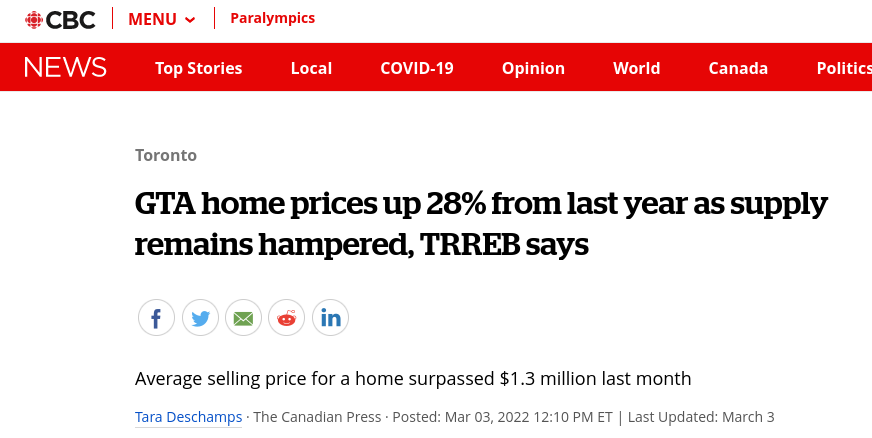
\includegraphics[width=12cm]{images/cbc_article.png} \\
    Source: \parencite{deschamps_2022}
\end{frame}

\begin{frame}
    \frametitle{Motivation}
    Average housing prices in Canada have increased $16\%$ since the beginning of the pandemic. This period also coincided with aggressive monetary and fiscal stimulus. \\
    \begin{figure}
        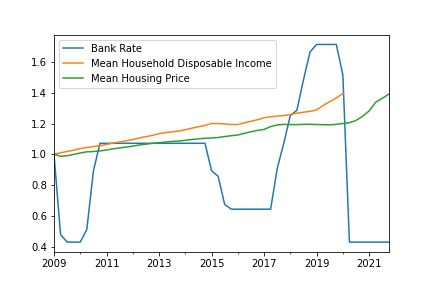
\includegraphics[height=4.5cm]{images/canada_housing.png}
        \centering 
    \end{figure}
    Note: Values shown are indices (Q1 2009 = 1). \\
    Source: \parencite{statcan}
\end{frame}

\begin{frame}
    \frametitle{Motivation}
    \begin{figure}
        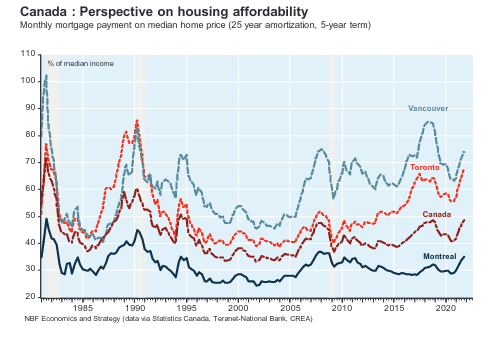
\includegraphics[height=6cm]{images/housing_affordability.png} 
        \centering   
    \end{figure}
    Source: \parencite{dahms_duchame_2022}
\end{frame}

\begin{frame}
    \frametitle{Motivation}
    \begin{figure}
        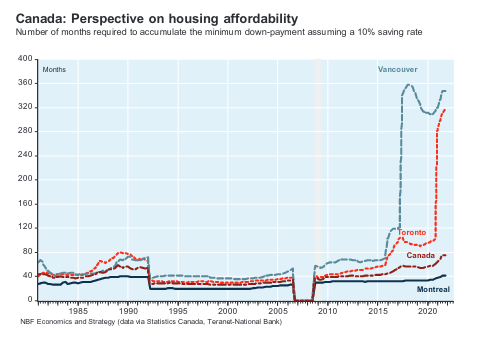
\includegraphics[height=6cm]{images/downpayment_time.png}
        \centering
    \end{figure}
    Source: \parencite{dahms_duchame_2022}
\end{frame}

\begin{frame}
    \frametitle{Question}
    \begin{itemize}
        \item What effect does monetary policy have on the affordability of housing and in particular, the affordability of housing deposits?
        \item Can housing affordability feed back into the effectiveness of monetary policy action in the future?
    \end{itemize}
\end{frame}

\begin{frame}
    \frametitle{Model}
    \begin{itemize}
        \item I will consider a model where a minimum down-payment must be made in order to enter the housing market.
        \begin{itemize}
            \item Can interpret this as meaning there is a minimum size of house that is available for purchase.
        \end{itemize}
        \item Results in two types of agents: homeowners and renters.
        \item Will use an OLG structure in order to have interesting transition between the two types.
        \item First start with a very simple model: endowment economy, two periods, supply of housing and consumption goods fixed at 1 (partial equilibrium).
    \end{itemize}
\end{frame}

\begin{frame}
    \frametitle{Setup}
    \begin{itemize}
        \item Agents live for two periods: $t=0,1$ and in each period a unit mass of agents are born.
        \item In period $0$ agents obtain an endowment drawn from $U(0, 1)$. In period $1$ their only income is their savings from period $0$.
        \item Renters can save only cash and are thus subject to uninsurable inflation risk. On the other hand homeowners have access to saving in both housing and bonds. Therefore, being a homeowner is a strictly better state for an agent.
        \item No arbitrage implies that the return on housing is equal to the return on bonds $(1+i_t)$. It is assumed that in equilibrium the homeowners actually hold no bonds.
        \item Agents become homeowners if their endowment is greater than the minimum down-payment $\phi p^a_t$. Where $\phi$ is a constant and $p^a_t$ is the housing price.
    \end{itemize}
\end{frame}

\begin{frame}
    \frametitle{Renter Problem}
    \begin{align}
        \underset{c^r_{t|t}, c^r_{t+1|t}, h^r_{t|t}, h^r_{t+1|t}, \omega_{t+1|t}}{\max} &ln(c^r_{t|t}) + ln(h^r_{t|t}) + \beta[ln(c^r_{t+1|t}) + ln(h^r_{t+1|t})] \nonumber \\
        \text{s.t. }& \omega_{t|t} = c^r_{t|t} + r_{t}^h h^r_{t|t} + \omega_{t+1|t} \nonumber \\
        & \omega_{t+1|t} = \mathbb{E}_t(p_{t+1})c^r_{t+1|t} + \mathbb{E}_t(r^h_{t+1})h^r_{t+1|t}
    \end{align}
\end{frame}

\begin{frame}
    \frametitle{Homeowner Problem}
    \begin{align}
        &\underset{c^o_{t|t}, c^o_{t+1|t}, h_{t|t}, h_{t+1|t}, a_{t|t}, b_{t|t}}{\max} ln(c^o_{t|t}) + ln(h_{t|t}) + \beta[ln(c^o_{t+1|t}) + ln(h_{t+1|t})] \nonumber \\
        \text{s.t. }& \omega_{t|t} + r^a_t(a_{t|t} - h_{t|t}) = c^o_{t|t} + p^a_t (1 + i_t) a_{t|t} + b_{t|t} \nonumber \\
        & (1 + i_t) b_{t|t} + \mathbb{E}_t (p^a_{t+1}) a_{t|t} = \mathbb{E}_t(p_{t+1})c^o_{t+1|t} + \mathbb{E}_t(r^a_{t+1})h_{t+1|t}
    \end{align}
\end{frame}

\begin{frame}
    \frametitle{Results}
    \begin{align}
        \bar{p}^a =& \frac{1 + \bar{i}}{\bar{i}(1 + \beta(1 + \bar{i}))} \label{ss_housing_price} \\
        \hat{c}_{t+1} =& (1-\frac{1}{2} \phi \bar{p}^a)(1 +\hat{i} - \mathbb{E}_t (\pi_{t+1})) \hat{c}^o_{t|t} \nonumber \\
        +& \frac{\beta \phi \bar{p^a}}{2(1+\beta)} (1 - \mathbb{E}_t(\pi_{t+1})) \hat{c}^r_{t|t} \nonumber \\
        +& \frac{1-\frac{1}{2} \phi \bar{p}^a}{1 + \beta(1+\bar{i})} \hat{c}^o_{t+1|t+1} \nonumber \\
        +& \frac{\phi \bar{p^a}}{2(1+\beta)} \hat{c}^r_{t+1|t+1} \label{is_equation}
    \end{align}
\end{frame}

\begin{frame}
    \frametitle{Results}
    \begin{figure}
        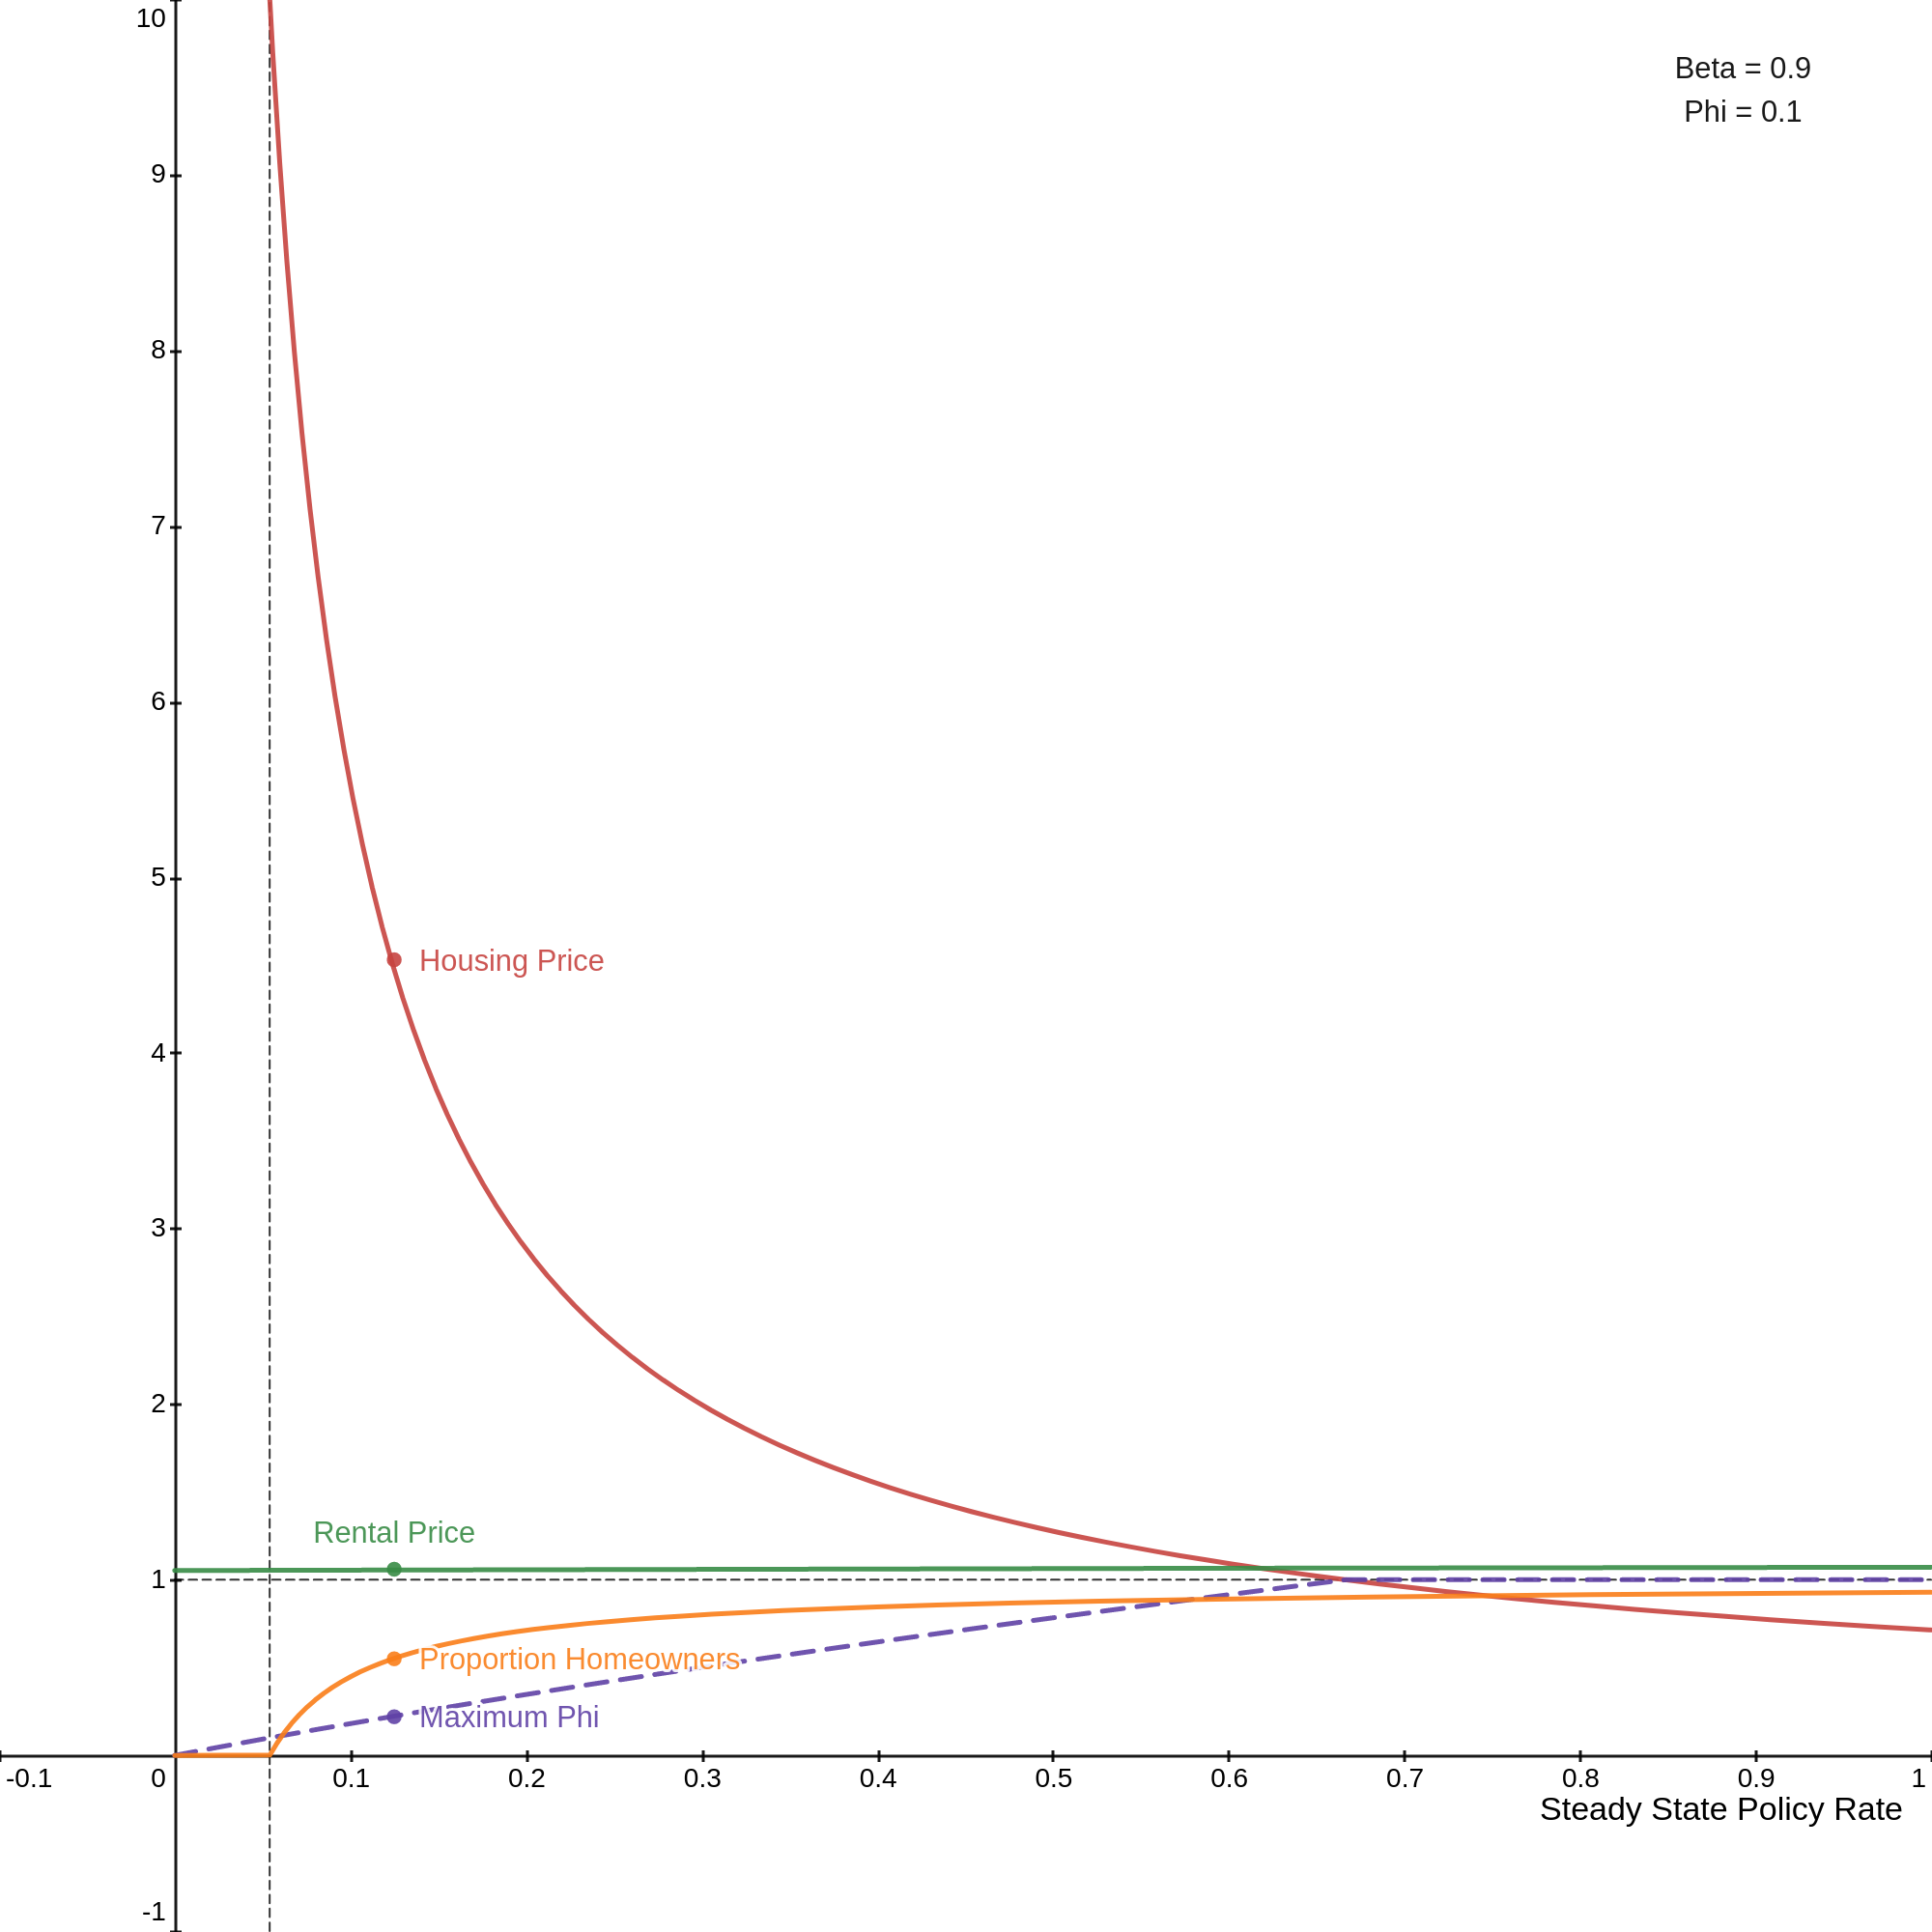
\includegraphics[height=8cm]{images/asset_price_rental_rate.png}
        \centering
    \end{figure}
\end{frame}

\begin{frame}
    \frametitle{Interpretation}
    \begin{itemize}
        \item Interest rates are related to the cost of homeownership.
        \item Therefore, lower (steady-state) rates raise demand for housing.
        \item However, since supply is fixed, this translates directly into increased housing prices.
        \item Due to minimum down-payment higher prices result in lower homeownership.
        \item Since homeowners are directly affected by monetary policy, and renters are not, lower steady state interest rates result in a weaker response to monetary policy shocks via IS equation.
    \end{itemize}
\end{frame}

\begin{frame}
    \frametitle{Problem}
    \begin{itemize}
        \item This analysis is only partial equilibrium. In order to see how shocks propagate through the system we need to move to general equilibrium framework. 
        \item Unfortunately, we already have to leave the analytically tractable world at this point, even in steady state.
        \item In order for supply to respond to demand (IS equation) there has to be endogenous labour supply. But then the agents could manipulate their labour supply to affect their type $\implies$ heterogeneous and non-linear response.
        \item Because of the high-dimensional and non-linear nature of this problem, traditional simulation techniques may perform poorly \parencite{han2021deepham}.
    \end{itemize}
\end{frame}

\begin{frame}
    \frametitle{Solution}
    \centering{Machine Learning!}
    \vspace{0.5cm}
    \begin{itemize}
        \item I will use the approach of \citeauthor{maliar2021deep} (\citeyear{maliar2021deep}) and \citeauthor{azinovic2019deep} (\citeyear{azinovic2019deep}) in order to estimate the equilibrium policy functions in a much more complicated (and realistic) version of the baseline model.
        \item Use neural networks because they are known to be useful for estimating non-linear functions in high-dimensional spaces. Neural networks are known to be able to overcome the curse of dimensionality \parencite{shen2021neural}.
        \item Usual downsides (overfitting, interpretability) are less relevant; in this context we are only interested in functional approximation. Indeed, sufficiently large neural networks can approximate any (measurable) function \parencite{hornik1989multilayer}.
    \end{itemize}
\end{frame}

\begin{frame}
    \frametitle{Machine Learning Solution Method}
    \begin{itemize}
        \item Abstractly, the process of estimating a macroeconomic equilibrium can be thought of as the process of estimating the optimal policy functions (control variables) (and in some cases the value function) of agents conditional on (1) states, (2) shocks, and (3) expectations. 
        \item Once policy functions are known the state transition is implied by the resource constraints of the economy. Using this we can observe how shocks propagate (e.g. impulse response functions).
        \item Instead of perturbation or projection I will parameterize the policy functions as a neural network:
    \end{itemize}

    \vspace{-0.5cm}

    \begin{equation}
        \psi(X_t, \epsilon_t; \theta) = \sigma_k(... \sigma_1(W_1\sigma_0(W_0\left[X_t, \epsilon_t\right]^T + b_0) + b_1) ... + b_k)
    \end{equation}

    \begin{itemize}
        \item Where $\sigma_i$ are activation functions for each layer, and $W_i$ and $b_i$ are weight and bias parameters for each layer. 
    \end{itemize}
    
\end{frame}

\begin{frame}
    \frametitle{Estimation (In General)}
    \begin{itemize}
        \item In order to estimate the parameters of the neural network start from some initial guess ($\theta_0$), then iteratively improve the estimate of the parameters by moving the parameters some amount ($\alpha_t$) against the direction of the gradient. This process is known as Stochastic Gradient Descent (SGD).
        \item In particular, we use the gradient of a "loss function" ($L$) which indicates the quality of our estimate.
        \item In each step we use a different randomly selected sample of data known as a "batch" ($b$). This is what makes the process "stochastic".
    \end{itemize}
    
    \begin{equation}
        \theta_{t+1} = \theta_{t} - \alpha_t \nabla_\theta \left[\frac{1}{|b|} \sum_{i \in b} L(X_i, \epsilon_i; \theta_t)\right]
    \end{equation}

    \begin{itemize}
        \item Calculation of the gradient is feasible due to a computational technique known as \textit{back-propogation}.
    \end{itemize}
\end{frame}

\begin{frame}
    \frametitle{Estimation (Details)}
    \begin{itemize}
        \item When solving macroeconomic models the loss is a sum of the (squared) deviations from the optimality conditions of the economic model (first order conditions, Euler equations, Bellman equations, etc).
        \begin{itemize}
            \item If the first order condition is $U_c(c_t,...) = \lambda_t$ then the corresponding component of the loss would be $(U_c(\hat{c}_t,...) - \hat{\lambda}_t)^2$
            \item When dealing with a value function we want the LHS and RHS of the Bellman equation to be similar, so we add the penalty: $\left(\frac{U(.) + V_1(.)}{V_0(.)} - 1\right)^2$
        \end{itemize}
        \item When the optimal choices involve expectations we integrate over the distribution of shocks by replacing the square with the product of the loss components for two independent draws of future shocks \parencite{maliar2021deep}. By eliminating the covariance term in this way (orthogonality) we maintain the unbiasedness of the batch loss.
    \end{itemize}
\end{frame}

\begin{frame}
    \frametitle{Estimation (More Details)}
    \begin{itemize}
        \item In high dimensional state spaces it is impractical to draw states randomly as it would take too long for the sampled states to adequately cover the entire state space. This is one cause of the curse of dimensionality \parencite{bellman1961curse}.
        \item Instead, we can use the state transition implied by our current model estimate to sample from the \textit{ergodic set} of the equilibrium. This has the effect of estimating the parameters exactly on the manifold that the states will lie on in equilibrium, which is usually dramatically smaller than the entire state-space \parencite{judd2011numerically}.
        \item Therefore, the estimation procedure is as follows:
        \begin{enumerate}
            \item Begin with some initial parameter guess ($\theta_0$) and random sample from the state space ($X_0$). 
            \item Update parameter estimate to $\theta_1$ via SGD over $X_0$.
            \item Update the sample of states to $X_1$ using the state transition $X_0$ implied by $\psi(X_0, \epsilon_0; \theta_0)$ and random draws from the distribution of $\epsilon$. Iterate forward sufficiently that it is plausible that $X_1 \indep X_0$.
            \item Repeat...
        \end{enumerate}
    \end{itemize}
\end{frame}

\begin{frame}
    \frametitle{Model (Revisited)}
    \begin{itemize}
        \item Currently I am working on estimating the following model using these ML techniques.
        \item Consumption goods supplied by firms in monopolistic competition with Calvo pricing \parencite{calvo1983staggered} as is standard in New Keynesian models. Supply of housing still fixed at $1$.
        \item Overlapping generations of agents live for $T$ periods and solve the following maximization problem in each period:
    \end{itemize}
    \begin{align}
        V(m_{t-1}, a_{t-1}, b_{t-1}, o_{t-1}, t) =& \max \{ U(c_t, h_t, 1-n_t) \nonumber \\
        +& \beta \mathbf{1}(.) V(0, a_t, b_t, 1, t+1) \nonumber \\
        +& \beta (1 - \mathbf{1}(.)) V(m_t, 0, 0, 0, t+1) \} \\
        \text{s.t. }& c_t + p^a_t (a_t - a_{t-1}) + r^h_t h_t + b_t + m_t \nonumber \\
        =& r^h_ta_{t-1} + \frac{1}{1+\pi_t}((1+i_t) b_{t-1} + m_{t-1}) \\
        &\mathbf{1}(.) = \mathbf{1}(\{m_{t-1} > \phi p^a_t\} \cup \{o_{t-1} = 1\}) \\
        & a_T = m_T = b_T = 0
    \end{align}
\end{frame}

\begin{frame}
    \frametitle{Next Steps}
    \begin{itemize}
        \item Actually get estimation to produce sensible results for single agent case.
        \item Add general equilibrium features (production, overlapping generations, estimation of equilibrium prices, stochastic shocks).
        \item Add bells and whistles (e.g. cashflow constraint forces homeowners to liquidate, homeowners hold cash in equilibrium).
        \item Calibrate model to try and ascertain how important this mechanism is in reality.
    \end{itemize}
\end{frame}

\begin{frame}
    \centering{Questions?}
\end{frame}

\begin{frame}
    \printbibliography
\end{frame}

\end{document}